% Ensure that you compile using XeLaTeX !!! PDFTex has problems with some of the packages used
\documentclass[12pt]{article}
\setlength\parindent{0pt}

\usepackage{parskip}
\usepackage[margin=0.5in]{geometry}
\usepackage{fullpage}
\usepackage{moresize}
\usepackage{graphicx}
\usepackage{caption}
\usepackage{subcaption}
\usepackage{float}
\usepackage{xcolor}
\usepackage{soul}
\usepackage{fontspec}
\setmainfont{Doulos SIL}

\begin{document}

\begin{center}
\textbf{{\color{violet}{\HUGE 20201028 Wednesday\\}}}

\textbf{{\color{violet}{\HUGE ALL EXAMS\\}}}

\end{center}
\newpage

\begin{center}
\textbf{{\color{blue}{\HUGE START OF EXAM\\}}}

\textbf{{\color{blue}{\HUGE Student ID: empty\\}}}

\textbf{{\color{blue}{\HUGE 10:00\\}}}

\end{center}
\newpage

\begin{center}
\textbf{{\color{blue}{\HUGE START OF EXAM\\}}}

\textbf{{\color{blue}{\HUGE Student ID: 36116\\}}}

\textbf{{\color{blue}{\HUGE 10:10\\}}}

\end{center}
\newpage

{\large Question 1}\\

Topic: Skewed Distributions\\
Source: Week 5 Handout, Question 6\\

If I gave you a new word in Malto, [di\_\_u], would it be possible to predict whether it's [d] or [t] that goes in the blank? Explain why or why not.\\

\begin{figure}[H]
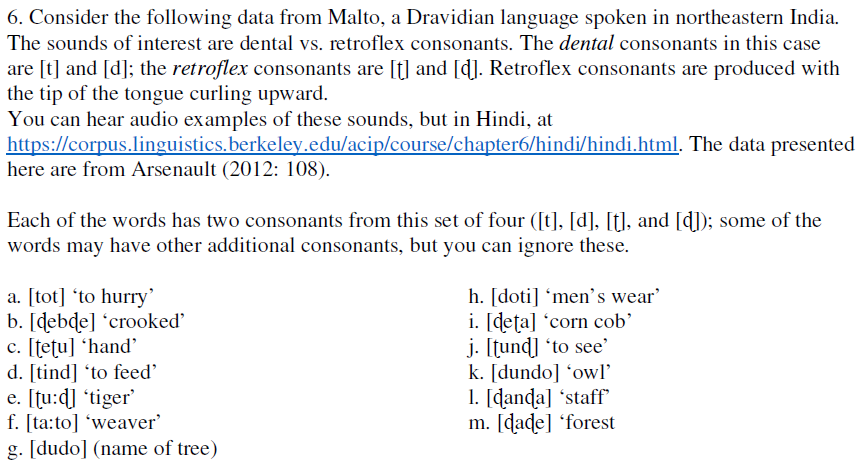
\includegraphics{../images/malto.png}
\end{figure}

\newpage

{\large Question 2}\\

Topic: Other (pre-midterm)\\
Source: Week 4 Handout, Part II, Question 2(iv)\\

Explain how you would figure out the Swahili word for this English gloss. (To be clear: you do NOT need to give me the Swahili form itself -- just explain the process of figuring it out.)\\

‘They will pay him.’

\begin{figure}[H]
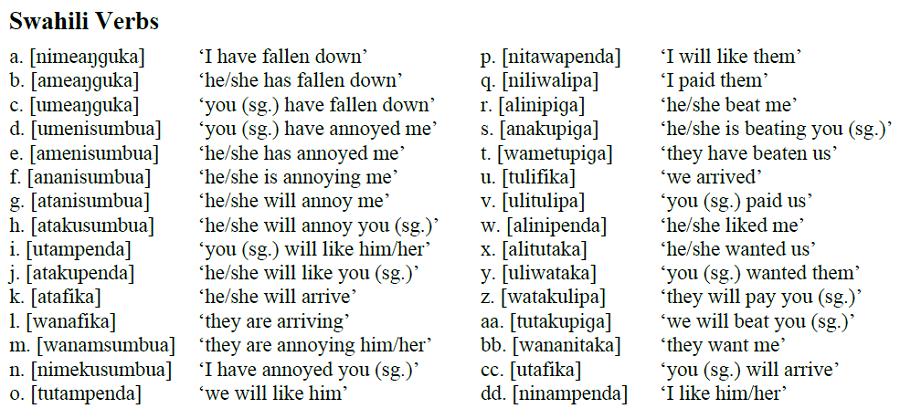
\includegraphics{../images/swahiliverbs.png}
\end{figure}

\newpage

\begin{center}
\textbf{{\color{red}{\HUGE END OF EXAM}}}\\

\end{center}
\newpage

\begin{center}
\textbf{{\color{blue}{\HUGE START OF EXAM\\}}}

\textbf{{\color{blue}{\HUGE Student ID: 83841\\}}}

\textbf{{\color{blue}{\HUGE 10:20\\}}}

\end{center}
\newpage

{\large Question 1}\\

Topic: Transcription\\
Source: Week 2 Handout, Part II\\

Is this a reasonable transcription of this word? Explain why.\\

<paid>: {[peid]}


\newpage

{\large Question 2}\\

Topic: Articulatory Phonetics\\
Source: Week 3 Handout, Question 9\\

Explain how to figure out what the sound being produced is in this diagram.\\

\begin{figure}[H]
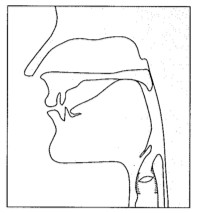
\includegraphics{../images/sagittal_k.png}
\end{figure}

\newpage

\begin{center}
\textbf{{\color{red}{\HUGE END OF EXAM}}}\\

\end{center}
\newpage

\begin{center}
\textbf{{\color{blue}{\HUGE START OF EXAM\\}}}

\textbf{{\color{blue}{\HUGE Student ID: 74752\\}}}

\textbf{{\color{blue}{\HUGE 10:30\\}}}

\end{center}
\newpage

{\large Question 1}\\

Topic: Skewed Distributions\\
Source: Week 5 Handout, Question 3\\

What evidence is there that there is a pattern in these data, assuming that these are the only CV and VC sequences that occur in some language?\\

{[sa]}, {[ʃi]}, {[za]}, {[ʒi]}, {[as]}, {[iʃ]}, {[az]}, {[iʒ]}


\newpage

{\large Question 2}\\

Topic: Other (pre-midterm)\\
Source: Week 5 \& 6 Handouts\\

Explain how you could analyze this dataset in terms of sequential patterns vs. paradigmatic patterns.\\

\begin{figure}[H]
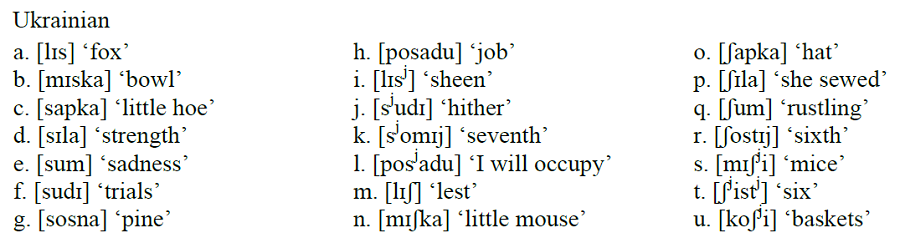
\includegraphics{../images/ukrainian.png}
\end{figure}

\newpage

\begin{center}
\textbf{{\color{red}{\HUGE END OF EXAM}}}\\

\end{center}
\newpage

\begin{center}
\textbf{{\color{blue}{\HUGE START OF EXAM\\}}}

\textbf{{\color{blue}{\HUGE Student ID: 17335\\}}}

\textbf{{\color{blue}{\HUGE 10:40\\}}}

\end{center}
\newpage

{\large Question 1}\\

Topic: Articulatory Phonetics\\
Source: Quiz 2, Question 7\\

Why might more than one of the descriptions given truthfully apply to the sound represented by the underlined letter, and why is one of them actually better than the other?\\

<a\underline{w}ay>

\begin{itemize} \item prevocalic obstruent \item prevocalic sonorant \item postvocalic obstruent \item postvocalic sonorant \item intervocalic obstruent \item intervocalic sonorant \end{itemize}


\newpage

{\large Question 2}\\

Topic: Skewed Distributions\\
Source: Week 5 Handout, Question 6\\

If I gave you a new word in Malto, [di\_\_u], would it be possible to predict whether it's [d] or [t] that goes in the blank? Explain why or why not.\\

\begin{figure}[H]
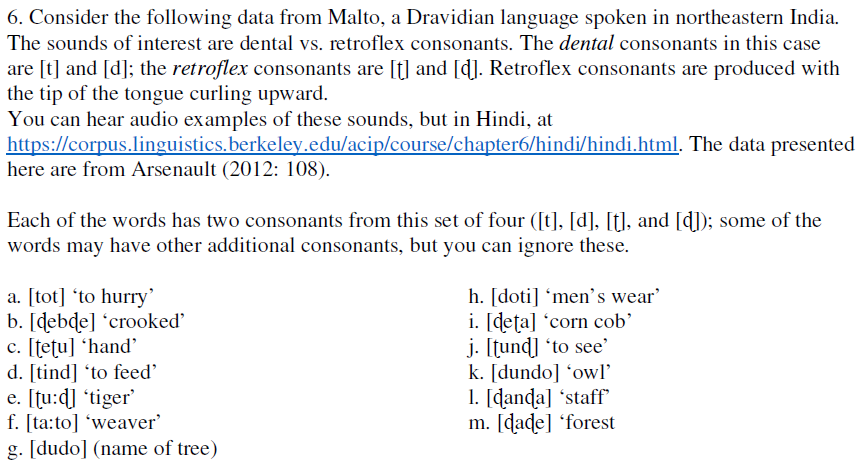
\includegraphics{../images/malto.png}
\end{figure}

\newpage

\begin{center}
\textbf{{\color{red}{\HUGE END OF EXAM}}}\\

\end{center}
\newpage

\begin{center}
\textbf{{\color{blue}{\HUGE START OF EXAM\\}}}

\textbf{{\color{blue}{\HUGE Student ID: empty\\}}}

\textbf{{\color{blue}{\HUGE 10:50\\}}}

\end{center}
\newpage

\begin{center}
\textbf{{\color{blue}{\HUGE START OF EXAM\\}}}

\textbf{{\color{blue}{\HUGE Student ID: 33446\\}}}

\textbf{{\color{blue}{\HUGE 4:00\\}}}

\end{center}
\newpage

{\large Question 1}\\

Topic: Skewed Distributions\\
Source: Quiz 4, Question 2\\

L$_X$ (Language X) has three vowels, [i], [a], and [u]. L$_X$ has tri-syllabic roots. If L$_X$ does not allow non-identical high vowels to co-occur, which one of the following tri-syllabic vocalic sequences do you predict to be unattested in L$_X$? Explain why.\\

\begin{itemize} \item {[u...i...a]} \item {[a...i...a]} \item {[u...u...a]} \item {[a...i...i]} \end{itemize}


\newpage

{\large Question 2}\\

Topic: Articulatory Phonetics\\
Source: Week 3 Handout, Question 3\\

Explain why the additional vowel below either does or does not belong in the phonetic natural class defined by the original set of SNAE vowels.\\

Original set: {[ɛ]}, {[ɪ]}, {[ʊ]}, {[ɔ]}

Addition: {[æ]}


\newpage

\begin{center}
\textbf{{\color{red}{\HUGE END OF EXAM}}}\\

\end{center}
\newpage

\begin{center}
\textbf{{\color{blue}{\HUGE START OF EXAM\\}}}

\textbf{{\color{blue}{\HUGE Student ID: 27762\\}}}

\textbf{{\color{blue}{\HUGE 4:10\\}}}

\end{center}
\newpage

{\large Question 1}\\

Topic: Phonological Features\\
Source: Quiz 3, Question 12\\

Explain how you figure out which feature is involved in the process of umlaut shown below.\\

\begin{figure}[H]
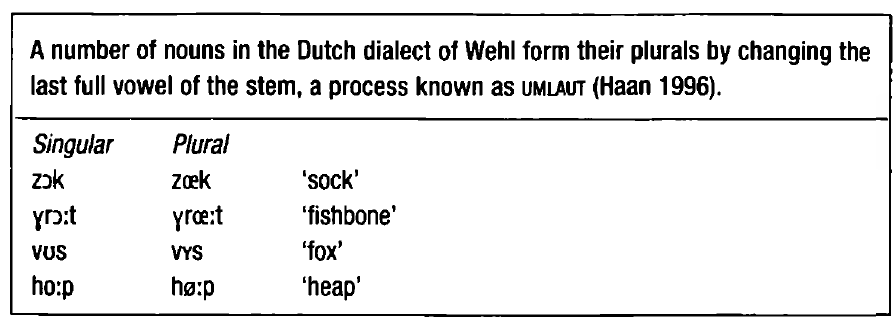
\includegraphics{../images/dutch.png}
\end{figure}

\newpage

{\large Question 2}\\

Topic: Skewed Distributions\\
Source: Quiz 4, Question 3\\

L$_X$ (Language X) has three vowels, [i], [a], and [u]. L$_X$ has tetra-syllabic roots. If L$_X$ does not allow non-identical high vowels to co-occur, which one of the following tetra-syllabic vocalic sequences do you predict to be unattested in L$_X$? Explain why.\\

\begin{itemize} \item {[i...i...u...u]} \item {[a...a...i...i]} \item {[u...u...u...u]} \item {[i...i...i...a]} \end{itemize}


\newpage

\begin{center}
\textbf{{\color{red}{\HUGE END OF EXAM}}}\\

\end{center}
\newpage

\begin{center}
\textbf{{\color{blue}{\HUGE START OF EXAM\\}}}

\textbf{{\color{blue}{\HUGE Student ID: 52421\\}}}

\textbf{{\color{blue}{\HUGE 4:20\\}}}

\end{center}
\newpage

{\large Question 1}\\

Topic: Transcription\\
Source: Week 2 Handout, Part II, Question 11\\

How would this word be transcribed?\\ (Kathleen will then ask a follow-up question about your transcription.)\\

<juice>


\newpage

{\large Question 2}\\

Topic: Skewed Distributions\\
Source: Week 5 Handout, Question 6\\

If I gave you a new word in Malto, [di\_\_u], would it be possible to predict whether it's [d] or [t] that goes in the blank? Explain why or why not.\\

\begin{figure}[H]
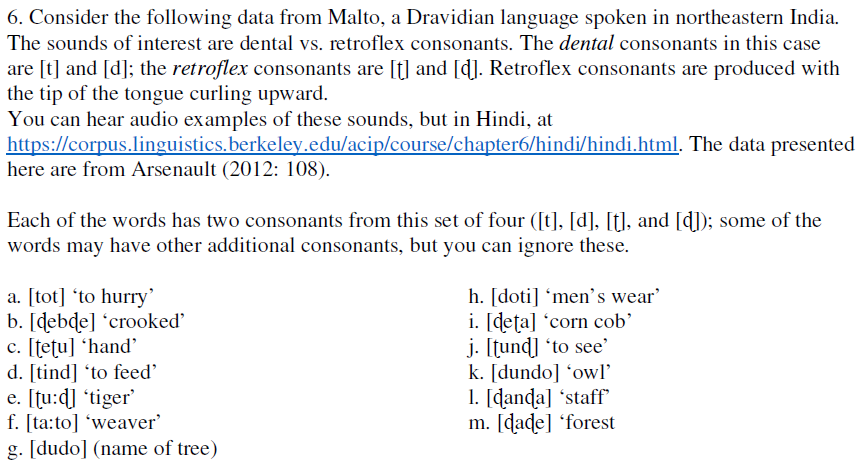
\includegraphics{../images/malto.png}
\end{figure}

\newpage

\begin{center}
\textbf{{\color{red}{\HUGE END OF EXAM}}}\\

\end{center}
\newpage

\begin{center}
\textbf{{\color{blue}{\HUGE START OF EXAM\\}}}

\textbf{{\color{blue}{\HUGE Student ID: 56567\\}}}

\textbf{{\color{blue}{\HUGE 4:30\\}}}

\end{center}
\newpage

{\large Question 1}\\

Topic: Skewed Distributions\\
Source: Week 5 Handout, Question 7\\

Explain how you would go about looking for co-occurrence restrictions in bi-syllabic signs in ASL. (Refer to the data that follows.)\\

\begin{figure}[H]
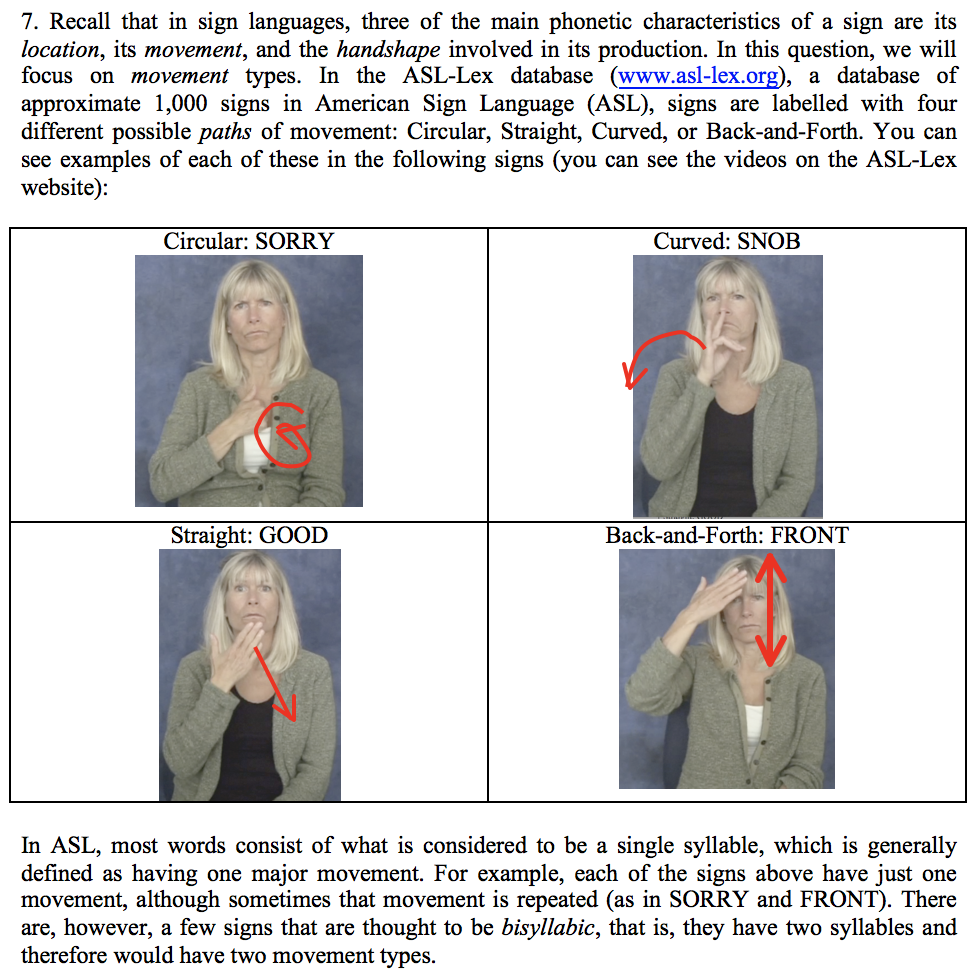
\includegraphics{../images/ASL_movement.png}
\end{figure}

\newpage

{\large Question 2}\\

Topic: Articulatory Phonetics\\
Source: Homework 1, Question 3(b)\\

Explain why this is or is not a complete phonetic natural class in standard North American English.\\

{[j]}, {[w]}


\newpage

\begin{center}
\textbf{{\color{red}{\HUGE END OF EXAM}}}\\

\end{center}
\newpage

\begin{center}
\textbf{{\color{blue}{\HUGE START OF EXAM\\}}}

\textbf{{\color{blue}{\HUGE Student ID: 36273\\}}}

\textbf{{\color{blue}{\HUGE 4:40\\}}}

\end{center}
\newpage

{\large Question 1}\\

Topic: Transcription\\
Source: Week 2 Handout, Part II\\

Is this a reasonable transcription of this word? Explain why.\\

<mouse>: {[mɔɪs]}


\newpage

{\large Question 2}\\

Topic: Other (pre-midterm)\\
Source: Week 4 Handout, Part II, Question 2(iv)\\

Explain how you would figure out the Swahili word for this English gloss. (To be clear: you do NOT need to give me the Swahili form itself -- just explain the process of figuring it out.)\\

‘I wanted them.’

\begin{figure}[H]
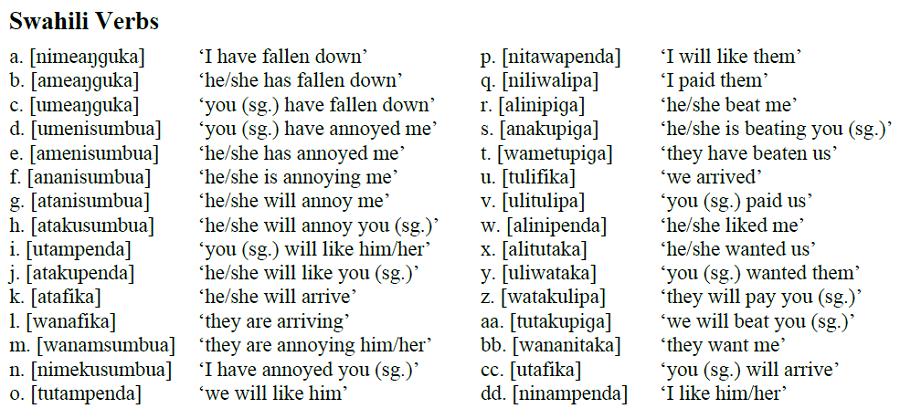
\includegraphics{../images/swahiliverbs.png}
\end{figure}

\newpage

\begin{center}
\textbf{{\color{red}{\HUGE END OF EXAM}}}\\

\end{center}
\newpage

\begin{center}
\textbf{{\color{blue}{\HUGE START OF EXAM\\}}}

\textbf{{\color{blue}{\HUGE Student ID: 19711\\}}}

\textbf{{\color{blue}{\HUGE 4:50\\}}}

\end{center}
\newpage

{\large Question 1}\\

Topic: Phonological Features\\
Source: Homework 2, Question 1\\

Explain which sound should be removed to make this a natural class (assuming SNAE, except that there are no diphthongs, no [ə] or [ʌ], no syllabic consonants, and no [w̥]), and what the minimum set of features would be to describe the resulting natural class.\\

{[i]}, {[ɪ]}, {[e]}, {[ɛ]}, {[æ]}, {[ɑ]}, {[ɔ]}, {[o]}, {[ʊ]}, {[u]}, {[ʒ]}, {[k]}, {[ɡ]}, {[ŋ]}, {[w]}


\newpage

{\large Question 2}\\

Topic: Skewed Distributions\\
Source: Week 5 Handout, Question 7\\

Explain how you would go about looking for co-occurrence restrictions in bi-syllabic signs in ASL. (Refer to the data that follows.)\\

\begin{figure}[H]
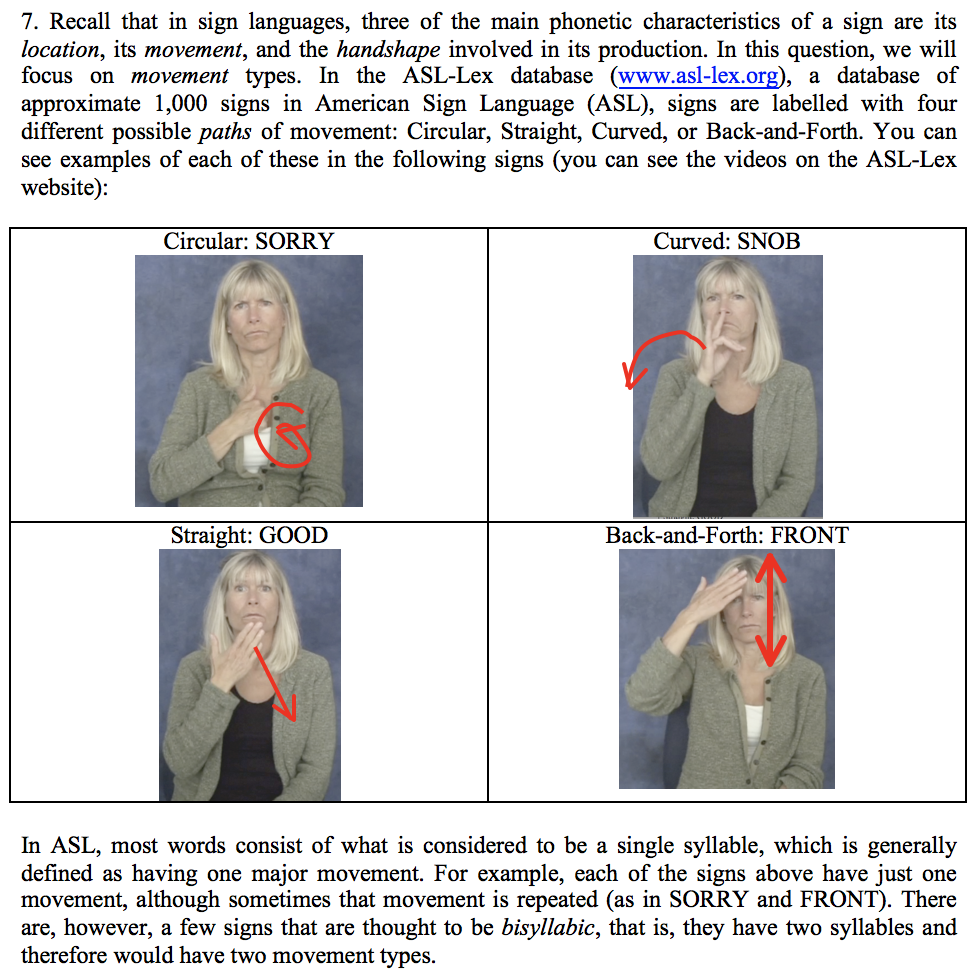
\includegraphics{../images/ASL_movement.png}
\end{figure}

\newpage

\begin{center}
\textbf{{\color{red}{\HUGE END OF EXAM}}}\\

\end{center}
\newpage

\end{document}

